\section{Approach}\label{sec:approach}

\todo[inline]{
    For the approach part, mention please also that it is open-source and where it can be found. Also, you keep the discussion around the implemented plant and the controller pretty short (and it is only showing up in the numerical part). Maybe it is better to discuss the details of the implemented plant and the controller already in Section 2 and mention that the intention is to build a liberary of plants and controllers in the future.
}

In this section, we present and detail our \ac{CLEAVE} framework for the performance evaluation of \acfp{NCS}, with a particular focus on edge deployments.
Our design follows an approach similar to the above-discussed \emph{hardware-in-the-loop} setups, in that we provide a \emph{framework} for the real-time \emph{emulation} of physical control systems which interact with \emph{real} networks.
This allows for great flexibility when it comes to the components of the control system, as these can easily be switched out in the fully emulated approach, while maintaining the realism of arguably the most complex and limiting component of and edge \acp{NCS}, namely the network itself.

In the following we will explain the approach taken in \ac{CLEAVE} by walking the reader through the steps necessary to deploy an arbitrary \ac{NCS} emulation on top of the framework.
An overview of the structure of such an emulation on \ac{CLEAVE} can be seen in \cref{fig:cleave:ncs:struct}.

\begin{figure*}
    \centering
    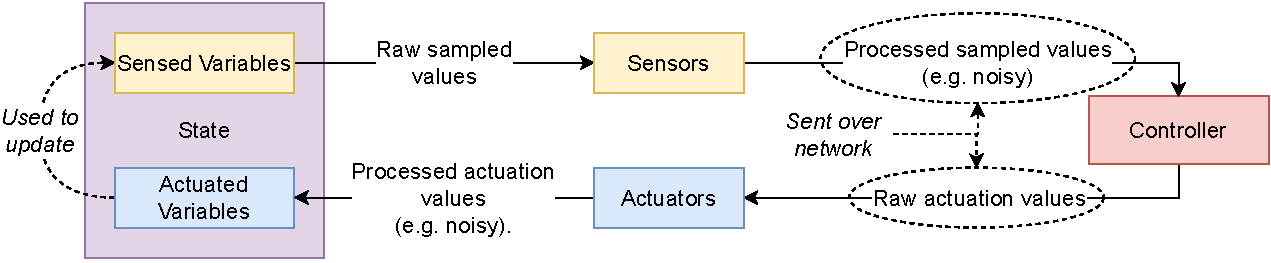
\includegraphics[width=.8\textwidth]{CLEAVE_NCS_structure}
    \caption{
        Structure of an emulated \ac{NCS} on top of CLEAVE.\@
        The State object implements the discrete-time evolution of the Plant.
        For this purpose, it holds two sets of special variables; Actuated Variables and Sensed Variables.
        Actuated Variables are updated from the values obtained from the Actuator objects at the beginning of each time step.
        These are used to perform a time step update in the State, and update the values of the Sensed Variables.
        The values of the Sensed Variables are then, at the end of each time step, sampled and passed on to the Sensor objects, which in turn process them (for instance, to add noise) and send the processed values to the Controller.
        The Controller uses these values to calculate the new actuation commands and sends these to the Actuators.
        Finally, the Actuators process the actuation commands and hold the new values for the Actuated Variables until they are read at the next time step.
    }\label{fig:cleave:ncs:struct}
\end{figure*}

\subsection{Defining a Plant}

The first step in developing an \ac{NCS} emulation on top of \ac{CLEAVE} is the definition of a Plant which represents the physical system to be controlled.

In abstract terms, Plants in \ac{CLEAVE} can be understood to be composed of
\begin{enumerate*}[itemjoin={{; }}, itemjoin*={{; and }}]
    \item\label{item:plant:state} an emulation of a physical system which is updated in a discrete-time fashion
    \item\label{item:plant:actuators} procedures to modify or act upon the physical emulation at each time-step
    \item\label{item:plant:sensors} procedures to sample relevant values from the physical emulation at each time-step
    \item\label{item:plant:network} procedures to interact with the network and send and receive data from the Controller.
\end{enumerate*}

While \cref{item:plant:network} is handled transparently by CLEAVE, by hiding it through layers of abstraction, the rest of the items need to be provided in more explicit ways by the user.

For \cref{item:plant:state}, the user needs to extend an abstract base class \texttt{State} provided by the framework.
This class provides the base functionality and defines a simple API for the implementation of discrete-time emulations by
\begin{enumerate*}[itemjoin={{; }}, itemjoin*={{; and }}]
    \item automatically tracking variables that can be modified and/or sampled by the framework
    \item defining a single abstract method \texttt{State.advance()} which is invoked by the framework on each time step of the emulation.
\end{enumerate*}

\Cref{item:plant:actuators,item:plant:sensors} are in the same way provided by the user through the extension of the \texttt{Actuator} and \texttt{Sensor} abstract base classes, respectively.
\texttt{Actuator} objects process the outputs of the Controller and update the values of the \texttt{State} accordingly.
Conversely \texttt{Sensor} objects sample relevant values from the \texttt{State} object, process them, and finally pass them on to the Controller through the network.

\subsection{Defining a Controller}

After the Plant has been defined, users need to implement a Controller for it.
This is once again done by extending an abstract base class, \texttt{Controller}, provided by CLEAVE.\@
This class defines a single abstract method, \texttt{Controller.process()} which is called by the framework whenever samples are provided by the Plant.
When invoked, it is passed a mapping of property names to sampled values.
The framework also expects implementations of this method to return yet another mapping, this time of actuated property names to target values.
Users are otherwise free to implement any kind of logic or process within extending classes.

\subsection{Configuring and running the emulation}

Once the core components for the emulation have been defined and implemented, the emulation needs to be configured to register them with the framework.
This is done through fully-featured Python scripts which simply define a number of required (and some optional) top-level variables.
An example of such a configuration file can be seen in \cref{lst:config:plant}.
These Python configuration files are then passed as arguments to the \texttt{cleave} bash command provided by the framework, which sets up and executes the emulation.
The use of Python scripts for configuration allows for a high degree of flexibility and complexity in the definition of emulation setups.

\begin{listing}
    \begin{minted}[linenos=true,
        breaklines, 
        breakafter=d,
        fontsize=\small]{Python}
from cleave.api.plant import SimpleConstantActuator, SimpleSensor
from cleave.impl.inverted_pendulum import InvPendulumState

# Plant emulation parameters
tick_rate = 100
emu_duration = '30m'
state = InvPendulumState(fail_angle_rad=0.34)
output_dir = './plant_metrics'

# Sensors to attach to the Plant
sensors = [
    SimpleSensor('position', 100),
    SimpleSensor('speed', 100),
    SimpleSensor('angle', 100),
    SimpleSensor('ang_vel', 100),
]

actuators = [
    SimpleConstantActuator(
        initial_value=0,
        prop_name='force')
]
    \end{minted}
    \caption{
        Example configuration file for a \ac{CLEAVE} Plant, defining the parameters for a single emulation.
        ``Plant emulation parameters'' define key emulation parameters, such as the emulation discrete-time update rate (the \emph{tick rate}).
        The Sensors and Actuators are then provided in lists, each Sensor and Actuator attached to a specific property identified by a string.
        Additionally, Sensors have a sampling rate in Hz which needs to be provided as an integer.
    }
    \label{lst:config:plant}
\end{listing}